\documentclass[10pt]{article}
\usepackage{fullpage}
\usepackage{amsfonts}
\usepackage{amsmath}
\usepackage{amsthm}
\usepackage{graphicx}
\usepackage{color}
\usepackage{amssymb}
\usepackage{empheq}
\usepackage{mathrsfs}
\usepackage{enumerate}
\usepackage{tikz}
\usepackage{pgflibraryarrows}
\usepackage{pgflibrarysnakes}
\usepackage{upgreek}
\usepackage{tipa}
\usepackage{multicol}
\usepackage{verbatim}
\usepackage{floatrow}
\usepackage{gensymb}
\usepackage{caption}

\usepackage{versions}
\excludeversion{sol}
\includeversion{sol}
\newenvironment{solution}{
\sol\\{\sc{Solution:}}}{
$\hfill\blacksquare$\endsol}

\def\|{||}
\def\R{\textbf{R}}
\def\C{\mathbb{C}}


\usepackage[T1]{fontenc}
\usepackage[font=small,labelfont=bf,tableposition=top]{caption}

\DeclareCaptionLabelFormat{andtable}{#1~#2  \&  \tablename~\thetable}

\newcommand{\pd}[2]{\frac{\partial #1}{\partial #2}}
\newcommand{\pdd}[2]{\frac{\partial^2 #1}{\partial {#2}^2}}
\newcommand{\pddd}[2]{\frac{\partial^3 #1}{\partial {#2}^3}}
\newcommand{\de}[2]{\frac{d #1}{d #2}}
\newcommand{\ppdd}[3]{\frac{\partial^2 #1}{\partial #2 \partial #3}}

\newtheorem*{1}{Problem 1}
\newtheorem*{2}{Problem 2}
\newtheorem*{3}{Problem 3}
\newtheorem*{4}{Problem 4}


\newfloatcommand{capbtabbox}{table}[][\FBwidth]

\usepackage{fancyhdr}
\setlength{\headheight}{15.2pt}
\pagestyle{fancy}
\setlength\headsep{30pt}
\lhead{P4.WS3 Worksheet}
\rhead{Kutztown University -- MATH 210}

\fancyfoot{}


%\rfoot{\tiny\textcopyright \textcolor{gray}{Brooks Emerick}}

\begin{document}

\begin{center}
\Large{\textsc{Phase 4 (part 3): 3-D Systems and 2$^{nd}$-Order Equations}}\\
\end{center}




%%%%%%%%%%%%%%%%%%%%%%%%%%%%%%%%%%%%%%%%%


\begin{enumerate}[{$\qquad 1.]$}]

\item An SIR model is a system of three differential equations that models the spread of an infectious disease throughout a population. Consider the compartment based model below and the associated system of equations. 
\begin{enumerate}
\item The classic endemic SIR model can be described by the following diagram:
\begin{center}
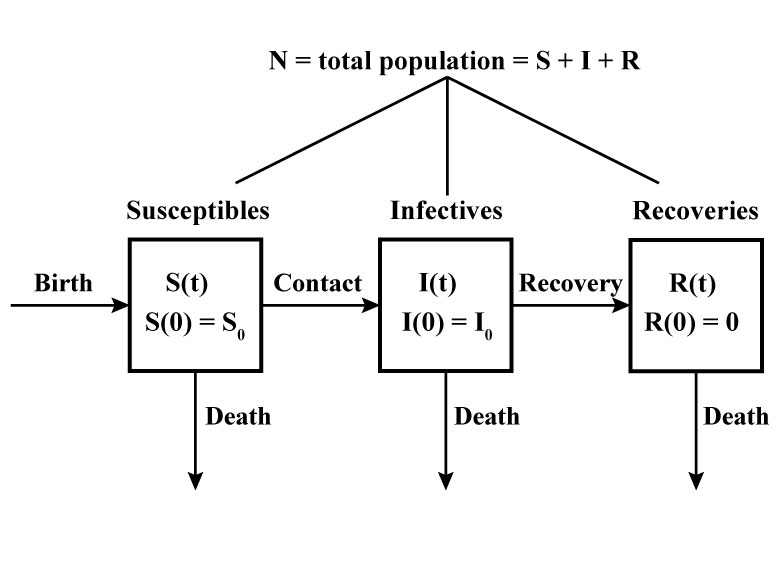
\includegraphics[width = .5\textwidth]{Infectious_Disease_3_web.jpg}
\end{center}
We can assemble the following equations based on this diagram:
\begin{align*}
\de{S}{t} & = \alpha N - \beta S \frac{I}{N} - \mu S\\
\de{I}{t} & =  \beta S \frac{I}{N}  - \gamma I- \mu I \\
\de{R}{t} & = \gamma I- \mu R \end{align*}
Here, $S_0$ and $I_0$ are the initial number of susceptible and infected persons at the beginning and the parameters $\alpha$, $\beta$, $\gamma$, and $\mu$ are the birth, incidence, recovery, and death rates, respectively.  $N$ is the total number of people in the population assumed constant. Solve this system for the following parameter values:
\begin{align*}
N  &    = 303824640 \\
\beta   &= 0.32851429\\
\mu     &= 0.00872\\
\alpha  &= 0.00872\\
\gamma & = 0.11673\end{align*}
with initial conditions, $I_0 = 1$, $R_0 = 0$, and $S_0 = N-1$, which means there is only one infected person in the whole population.  Once you solve the equations, plot the solutions on the same figure and change the incidence rate, $\beta$, to see what happens.  

\item Solve the system again but make the incidence rate $\beta$ a function of time of the form 
\[ \beta(t) = b_0 + b_1\sin(\pi t/6).\]
This simulates a periodic infectious rate that may change throughout a year.  It is up to you to decide the parameter values for $b_0$ and $b_1$.  

\end{enumerate}





\pagebreak 



\item The damped mass-on-a-spring system is modeled by the second-order differential equation 
\[ m \frac{d^2y}{dt^2} + b \frac{dy}{dt} + ky = kf(t), \] 
where $m>0$ is the mass, $b\geq 0$ is the damping coefficient, $k>0$ is the spring constant, $f(t)$ is a forcing function, and $y(t)$  is the displacement from equilibrium. This equation describes oscillatory motion where the damping force opposes the velocity, causing the oscillations to gradually decrease in amplitude over time.  Write this system as a first-order system of ODEs, then solve it in Python for various values of $m, b,$ and $k$ and for different forcing functions $f(t)$.  


\end{enumerate}

















\end{document}